%%%%%%%%%%%%%%%%%%%%%%%%%%%%%%%%%%%%%%%%%%%%%%%%%%%%%%%%%%%%%%%%%%%%%%%%%%%%%%%%%%%
%%%%%%%%%%%
%%%%%%%%%%% 494 participants 10-percentili
\begin{figure}
\centering

\ifx\USETIKZINFIGURE\undefined
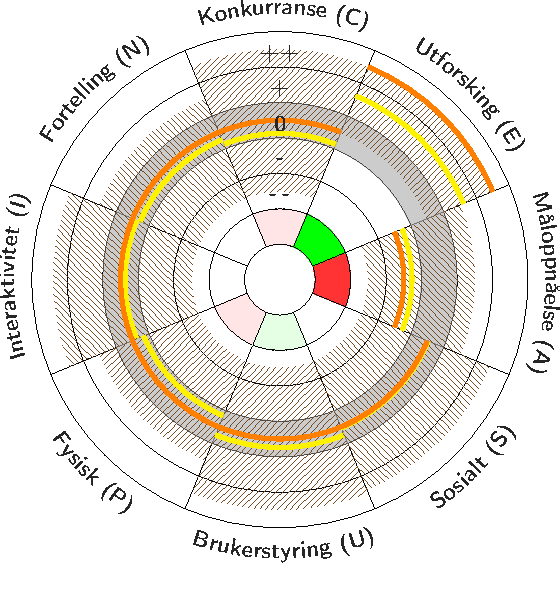
\includegraphics{figures/engagementikunior-112}
\else
\begin{tikzpicture}[scale=1.2]
\fontfamily{phv}\fontseries{mc}\selectfont
%\renewcommand{\CNIPUSNfontsize}{\normalsize}
\renewcommand{\CNIPUSNfontsize}{\small}
%\renewcommand*{\mytextstyle}{\fontfamily{phv}\fontseries{mc}\large\bfseries\color{black!85}}
%\renewcommand*{\myareatextstyle}{\fontfamily{phv}\fontseries{mc}\selectfont\footnotesize\color{black!85}}
%\renewcommand*{\mynumbertextstyle}{\fontfamily{phv}\fontseries{mc}\selectfont\large\bfseries\color{blue!85}}
\renewcommand{\CNIPUSNlabeladjustment}{-0.6mm}
\renewcommand{\CNIPUSNraise}{-0.5ex}

\path (\CNIPUSNL+\CNIPUSNLXX,\CNIPUSNL+\CNIPUSNLXX) --
(-\CNIPUSNL-\CNIPUSNLXX,\CNIPUSNL+\CNIPUSNLXX) --
(-\CNIPUSNL-\CNIPUSNLXX,-\CNIPUSNL-\CNIPUSNLXX-5mm) --
(\CNIPUSNL+\CNIPUSNLXX,-\CNIPUSNL-\CNIPUSNLXX-5mm);
%
% Draw background
\CNIPUSNdraw
% Draw labels
\CNIPUSNtext{xxx}{1}{Konkurranse (C)}
\CNIPUSNtext{xxx}{2}{Fortelling (N)}
\CNIPUSNtext{xxx}{3}{Interaktivitet (I)}
\CNIPUSNtext{xxx}{4}{Fysisk (P)}
\CNIPUSNtext{xxx}{5}{Brukerstyring (U)}
\CNIPUSNtext{xxx}{6}{Sosialt (S)}
\CNIPUSNtext{xxx}{7}{M{\aa}loppn{\aa}else (A)}
\CNIPUSNtext{xxx}{8}{Utforsking (E)}

% Draw in sector 1
\foreach \X in {1,2,...,8}{%
%\CNIPUSNdrawfill{fill=black}{\X}{0}
%\CNIPUSNdrawfill{fill=black!25!white}{\X}{3}
}

% Draw in sector 1C
\CNIPUSNfillborder{color=black!40!white, opacity=0.5}{1}{3}{3} % 0-ring
\CNIPUSNfillarea{pattern=north east lines, pattern color=brown!60!black}{1}{1}{5} % 3..4
\CNIPUSNline{color=yellow,line width=2pt}{1}{2.63}
\CNIPUSNline{color=orange,line width=2pt}{1}{3}
\CNIPUSNdrawfill{fill=white!90!red}{1}{0} 
%\CNIPUSNdrawfill{fill=white!1!green}{1}{0} % 43
% Formula: (x - 20)*3

% Draw in sector 2N
\CNIPUSNfillborder{color=black!40!white, opacity=0.5}{2}{3}{3} % 0-ring
\CNIPUSNfillarea{pattern=north west lines, pattern color=brown!60!black}{2}{1}{4} % 3..4
\CNIPUSNline{color=yellow,line width=2pt}{2}{2.77}
\CNIPUSNline{color=orange,line width=2pt}{2}{3}
%\CNIPUSNdrawfill{fill=white!20!blue}{2}{0}
%\CNIPUSNdrawfill{fill=white!84!green}{2}{0} % 61

% Draw in sector 3I
\CNIPUSNfillborder{color=black!40!white, opacity=0.5}{3}{3}{3} % 0-ring
\CNIPUSNfillarea{pattern=north west lines, pattern color=brown!60!black}{3}{1}{4.9} % 2.5 .. 4
\CNIPUSNline{color=yellow,line width=2pt}{3}{2.87}
\CNIPUSNline{color=orange,line width=2pt}{3}{3}
%\CNIPUSNdrawfill{fill=white!20!blue}{3}{0}
%\CNIPUSNdrawfill{fill=white!44!green}{3}{0} % 51

% Draw in sector 4P
\CNIPUSNfillborder{color=black!40!white, opacity=0.5}{4}{3}{3} % 0-ring
\CNIPUSNfillarea{pattern=north east lines, pattern color=brown!60!black}{4}{1}{4} % 3 .. 5
\CNIPUSNline{color=yellow,line width=2pt}{4}{2.66}
\CNIPUSNline{color=orange,line width=2pt}{4}{3}
\CNIPUSNdrawfill{fill=white!90!red}{4}{0}
%\CNIPUSNdrawfill{fill=white!1!green}{4}{0} % 40

% Draw in sector 5U
\CNIPUSNfillborder{color=black!40!white, opacity=0.5}{5}{3}{3} % 0-ring
\CNIPUSNfillarea{pattern=north east lines, pattern color=brown!60!black}{5}{1}{5} % 3 .. 5
\CNIPUSNline{color=orange,line width=2pt}{5}{3}
\CNIPUSNline{color=yellow,line width=2pt}{5}{3.24}
\CNIPUSNdrawfill{fill=white!90!green}{5}{0} % 47
%\CNIPUSNdrawfill{fill=white!28!green}{5}{0} % 47

% Draw in sector 6S
\CNIPUSNfillborder{color=black!40!white, opacity=0.5}{6}{3}{3} % 0-ring
\CNIPUSNfillarea{pattern=north west lines, pattern color=brown!60!black}{6}{1}{4.9} % 2 .. 4
\CNIPUSNline{color=yellow,line width=2pt}{6}{3.03}
\CNIPUSNline{color=orange,line width=2pt}{6}{3}
%\CNIPUSNdrawfill{fill=white!20!blue}{6}{0} 
%\CNIPUSNdrawfill{fill=white!84!green}{6}{0} % 61

% Draw in sector 7A
\CNIPUSNfillborder{color=black!40!white, opacity=0.5}{7}{3}{3} % 0-ring
\CNIPUSNfillarea{pattern=north west lines, pattern color=brown!60!black}{7}{1}{4} % 3 .. 4
\CNIPUSNline{color=orange,line width=2pt}{7}{2}
\CNIPUSNline{color=yellow,line width=2pt}{7}{2.23}
\CNIPUSNdrawfill{fill=white!20!red}{7}{0} 
%\CNIPUSNdrawfill{fill=white!32!green}{7}{0} % 48

% Draw in sector 8E
\CNIPUSNfillborder{color=black!40!white, opacity=0.5}{8}{3}{3} % 0-ring
\CNIPUSNfillarea{pattern=north east lines, pattern color=brown!60!black}{8}{3}{5} % 3 .. 4
\CNIPUSNline{color=orange,line width=2pt}{8}{5}
\CNIPUSNline{color=yellow,line width=2pt}{8}{4.11}
\CNIPUSNdrawfill{fill=white!1!green}{8}{0} % 61
%\CNIPUSNdrawfill{fill=white!84!green}{8}{0} % 61

%%all cyan lines
%\CNIPUSNline{color=cyan, line width=2pt}{1}{3.66}
%\CNIPUSNline{color=cyan, line width=2pt}{2}{3.26}
%\CNIPUSNline{color=cyan, line width=2pt}{3}{3.38}
%\CNIPUSNline{color=cyan, line width=2pt}{4}{3.65}
%\CNIPUSNline{color=cyan, line width=2pt}{5}{3.50}
%\CNIPUSNline{color=cyan, line width=2pt}{6}{3.19}
%\CNIPUSNline{color=cyan, line width=2pt}{7}{3.43}
%\CNIPUSNline{color=cyan, line width=2pt}{8}{3.30}



% colour formula: (value - 40) * 4

\node at (0,{\CNIPUSNR/\CNIPUSNU*(1+1.4)}) {\mytextstyle -\,-}; 
\node at (0,{\CNIPUSNR/\CNIPUSNU*(2+1.4)}) {\mytextstyle -}; 
\node at (0,{\CNIPUSNR/\CNIPUSNU*(3+1.4)}) {\mytextstyle 0}; 
\node at (0,{\CNIPUSNR/\CNIPUSNU*(4+1.4)}) {\mytextstyle +}; 
\node at (0,{\CNIPUSNR/\CNIPUSNU*(5+1.4)}) {\mytextstyle ++}; 

\renewcommand{\CNIPUSNfontsize}{\scriptsize} % set to original value

%\CNIPUSNnumbers{1}
\end{tikzpicture}
\fi

\caption{%
Engasjementsdiagram for app / digital plattform for
kunst i offentlige rom;
112 deltakere i aldersgruppen 60+. 
Skraveringer representerer svarene mellom 10\% og  90\%
percentilene; orange linjer: median-verdi; gule linjer: middelverdi.
Segmentene i midten viser om deltakerne {\o}nsker (gr{\o}nn) eller ikke
{\o}nsker (r{\o}dt) disse elementene.
\WVL{[dette er resultater fra et annet prosjekt -- vises kun som eksempel]}
}%
\label{fig:Opinion:112}
\end{figure}
%%%%%%%%%%%%%%%%%%%%%%%%%%%%%%%%%%%%%%%%%%%%%%%%%%%%%%%%%%%%%%%%%%%%%%%%%%%%%%%%
%%%%%%%%%%%%%%%%%%%%%%%%%%%%%%%%%%%%%%%%%%%%%%%%%%%%%%%%%%%%%%%%%%%%%%%%%%%%%%%%
